\chapter{Our proposal}
In this chapter, we propose a cross-language code clone detection system based
on supervised machine learning. Our system can learn to detect clones across
programming languages by learning from existing code clones pairs, and is
language agnostic in the sense that we use a normalized AST structure which can
be generated from any programming language using a parser into feed our system.
We also present how to generate the data that our system accepts as input to
detect clones, and describe the dataset that we created in order to train and
evaluate our system.
%
\section{\label{sec:proposal-overview}Overview}
As discussed in the shortcomings of current approaches to code clone detection
in~\ref{sssec:shortcomings}, current comparison-based approaches to code clone
detection do not fit cross-language clone detection, especially when the target
languages do not share a common intermediate representation.
To overcome this issue, we propose a supervised approach to code clone detection
where the system is not given directly information about how code fragments
should be compared to each other, but rather uses training data to learn what
kind of code fragments should be, or not, considered as clones.

Our system is composed of the following subsystems, which we will describe more
thoroughly in the following sections.
\begin{enumerate}
\item\label{it:sup-model} CC-Learner --- Supervised ML model to learn and predict code clones
\item\label{it:unsup-model} \lstinline{bigcode-embeddings} --- Unsupervised ML
  model to learn token vector representations
\item\label{it:bigcode-astgen} \lstinline{bigcode-astgen} --- Parser modules to
  transform source code to a common AST format
\item\label{it:bigcode-ast-tools} \lstinline{bigcode-ast-tools} --- Tools to
  transform with ASTs generated by \lstinline{bigcode-astgen}
\item\label{it:sup-scraper} CC-Fetcher --- Module to scrape data to train CC-Learner
\item\label{it:unsup-scraper} \lstinline{bigcode-fetcher} --- Module to scrape data to train \lstinline{bigcode-embeddings}
\end{enumerate}
Figure~\ref{fig:system-overview} shows a general overview of how our system
works.

\begin{figure}
  \centering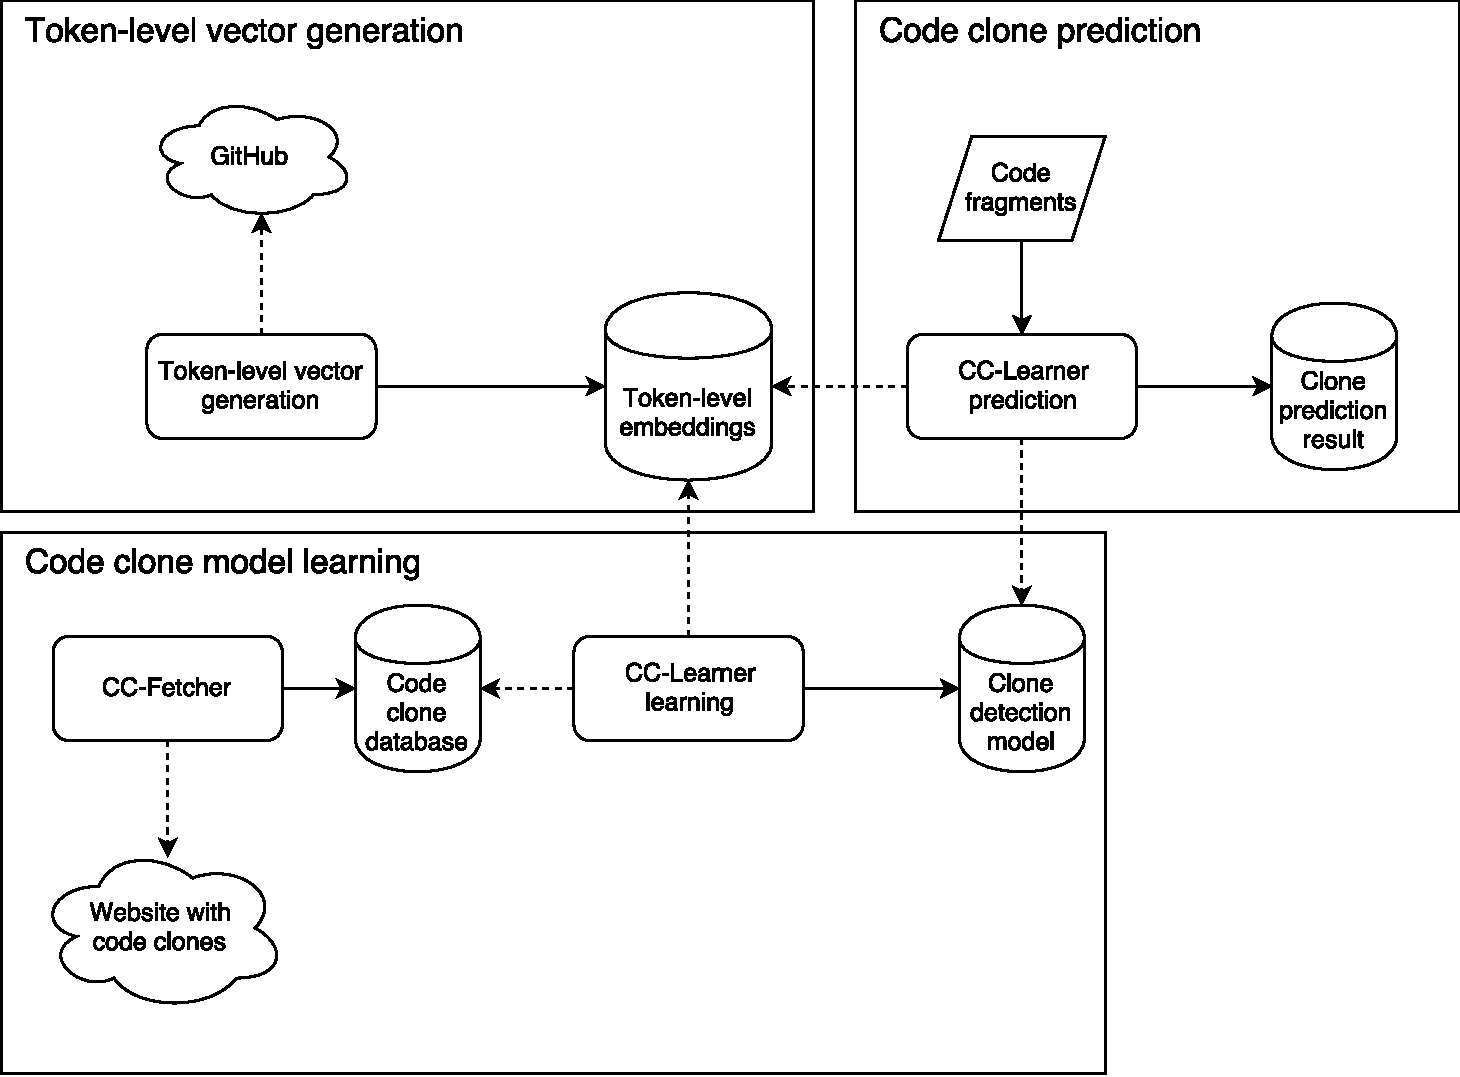
\includegraphics[width=13cm]{./images/system-overview.pdf}
  \caption{\label{fig:system-overview}Overview of the system}
\end{figure}

The core of our system is~\ref{it:sup-model}, which is an LSTM --- presented
in~\ref{ssec:rnn} --- base supervised machine learning model which takes two
code fragments as an input, and predict if the two code fragments are code
clones. The flow in training mode is to take two code fragments scraped
using the scraper module~\ref{it:sup-scraper}, transform the code pairs to ASTs
using the parser modules~\ref{it:bigcode-astgen}, transform the ASTs in to
vectors using the token representation learned by~\ref{it:unsup-model} and
finally to feed the result to our LSTM-based model~\ref{it:sup-model}.

In Section~\ref{sec:clone-detection}, we will describe in detail the model we
used to detect code clones. In Section~\ref{sec:ast-generation}, we will
describe the AST generation in order to be able to work with source code written
in different programming languages and in
Section~\ref{sec:token-representation}, we will explain how we assign a vector
in $\mathbb{R}^d$ to each token in the source code.
%
\section{\label{sec:clone-detection}Code clone detection model}
\subsection{Model overview}
The clone detection model, CC-Learner, that we first introduced in
Section~\ref{sec:proposal-overview} is the main of our system. Its main role is
to actually predict if two code fragments are, or not, clones. The model is
composed of the following components.
\begin{enumerate}
\item An AST to vector transformer
\item A token-level embedding layer
\item An LSTM-based encoder for AST vectors
\item A merge layer to concatenate the two code fragments vectors
\item A feed-forward neural network to make the code clone prediction
\end{enumerate}
%
Figure~\ref{fig:clone-detection-model} shows how these parts are connected
together.
%
\begin{figure}
  \centering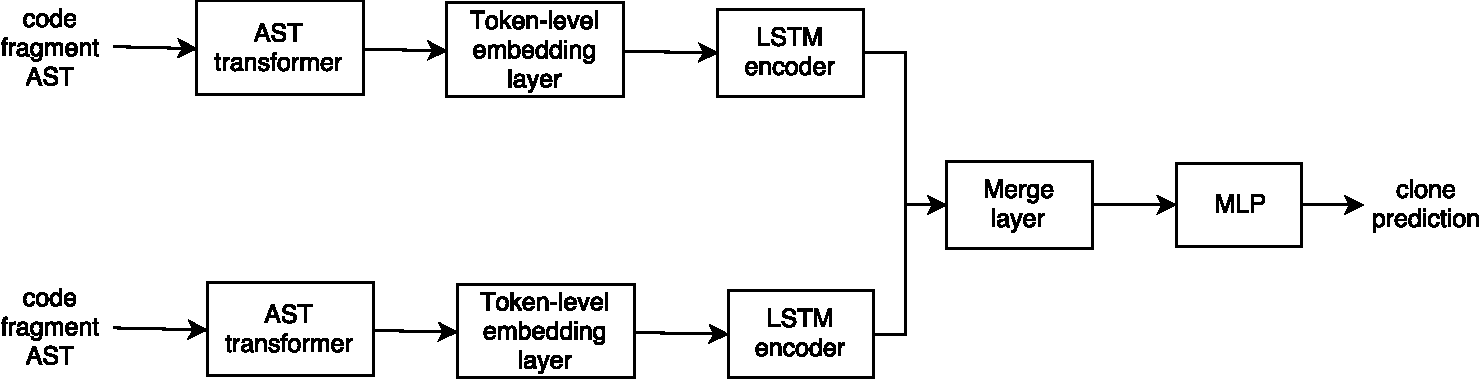
\includegraphics[width=16cm]{./images/model-overview.pdf}
  \caption{\label{fig:clone-detection-model}CC-Learner code clone detection model}
\end{figure}
%
In this section, we will first describe in details the computations done by the
model. We will then explain how we train the model, then how use the trained
model to predict if two code fragments are clones, and finally we will discuss
about the different hyper parameters of the models.
%
\subsection{Model computations}
We will here formalize the computations each component of the model executes to
produce the final prediction.
\subsubsection{AST to vector transformer}
As input, the model receives an AST, which is a tree structure. The AST to
vector transformer takes this AST and maps it into a vector of integers, where
each integer represents the index of the token in the AST in the vocabulary of
the programming language the source code is written in.

More formally, if we let $\mathcal{T}_l$ be the set of all possible ASTs for
source code written in programming language $l$, the AST transformer $f_t^l$ will
be a function with the following definition.

\begin{equation}
  f_t^l : \mathcal{T}_l \rightarrow \mathbb{N}^m
\end{equation}

where $m$ may vary depending on the size of the input tree and the algorithm
used for $f_t^l$. Furthermore, given $V_l$ is the vocabulary of tokens for the
programming language $l$, the following equation must hold for any
implementation of $f_t^l$.

\begin{equation}
  \forall t \in \mathcal{T}_l, n \in f_t^l(t), ~ n \in V_l
\end{equation}
%
For CC-Learner, we provide two different instances of this function, and the
function which is used is a hyper parameter of our model. We will use the code
snippet~\ref{lis:sample-snippet}, the AST of figure~\ref{fig:sample-ast} and the
vocabulary of table~\ref{tab:sample-vocabulary} to illustrate how both of our
instances work.
%
\begin{figure}
\begin{lstlisting}[language=Java,label=lis:sample-snippet,caption=Sample code snippet]
if (a < 1) {
  return 0;
}
\end{lstlisting}
\vspace*{1cm}
\end{figure}
%
\begin{figure}
  \centering\includedot[height=5cm]{./diagrams/sample-snippet.dot}
  \vspace*{-1cm}
  \caption{\label{fig:sample-ast} Sample AST}
\end{figure}
%
\begin{table}
  \caption{\label{tab:sample-vocabulary} Sample vocabulary}
  \begin{center}
    \begin{tabular}{cc}
      Token & Index\\
      \toprule%
      \ttfamily{if} & 1\\
      identifier & 2\\
      integer & 3\\
      \ttfamily{<} & 4\\
      \ttfamily{return} & 5\\
      \bottomrule%
    \end{tabular}
  \end{center}
\end{table}

The first instance of our AST to vector transformer is very simple. The idea is
simply to traverse the tree using a depth-first, pre-order tree traversal. At
each node in the tree, we look up the index of the node token in the vocabulary,
and we append the index to the output vector.

In our example above, the algorithm will start at the \lstinline{if} node, it
will lookup the index of the node in the vocabulary, which in this case is $1$,
and append $1$ to the output vector. It will then do the same thing with the
other nodes in the following order: \lstinline{<}, \lstinline{a}, \lstinline{1},
\lstinline{return}, \lstinline{0}. After completion, we will therefore obtain
the following vector in $\mathbb{N}^6$.
\begin{equation}
  \label{eq:sample-indexes-vector}
  \begin{pmatrix}1 & 4 & 2 & 3 & 5 & 3\end{pmatrix}
\end{equation}
When using this algorithm, the output dimension is always the same as the
number of nodes in the input AST.

Although the first instance of our AST to vector transformer is very simple and
straightforward, the main disadvantage is that it completely loses information
about the topology of the input tree. To mitigate this issue, we also
implemented another algorithm which tries to partially preserve the topology of
the tree in the output vector. In the above example, \lstinline{if} has two
children nodes: \lstinline{<} and \lstinline{return}, therefore the distance
inside the tree topology between \lstinline{if} and both of these nodes is $1$.
However, in the output vector, the distance between \lstinline{if} and
\lstinline{<} is $1$, but the distance between \lstinline{if} and
\lstinline{return} is $4$. For such a simple case, the distance is still short
enough for the neural to be able to capture relationship between these elements,
but in more complex cases, a distance of $1$ inside the tree topology could
easily become extremely large. This is the main issue we try to tackle with our
other instance of the AST to vector transformer function. The idea is to perform
a depth-first, pre-order traversal of the tree and generate the same vector as
in the first instance, but also to traverse the tree once more this time using a
depth-first, pre-order traversal but selecting the nodes from right to left
instead of selecting them from left to right when executing the traversal. Using
the above example, this means that in the second traversal, after visiting
\lstinline{if}, instead of visiting \lstinline{<}, we visit \lstinline{return}.
The second traversal order would therefore be \lstinline{if},
\lstinline{return}, \lstinline{0}, \lstinline{<}, \lstinline{1}, \lstinline{a}.
Once we have finished traversing the AST in both direction, we concatenate the
vectors obtain by each traversal to obtain the final vector for the AST. For the
above example, the final vector will be

\[ \begin{pmatrix}1 & 4 & 2 & 3 & 5 & 3 & 1 & 5 & 3 & 4 & 3 & 2\end{pmatrix} \]

As we are concatenating two vectors generated by a full traversal of the tree,
and which will therefore each have the dimension of the number of nodes in the
tree, the final output vector will have twice the dimension of the number of
nodes in the tree. Therefore, if there are $n$ nodes in the tree, the output
will be a vector in $\mathbb{N}^{2n}$.
%
\subsubsection{Token-level embedding layer}
When we transform an AST in to a vector using the above approach, we obtain a
vector of indexes. As each index cannot be fed directly to the encoder, the two
main approaches are to use a one-hot vector for the index, or to use a
distributed vector representation. As using a distributed vector representation
has many advantages~\cite{DBLP:journals/corr/MikolovSCCD13} over using one-hot
vectors, we choose this approach for our model. We will here assume that we
already have the embedding for each token available, and will describe how we
actually compute these embedding in Section~\ref{sec:token-representation}.

The embedding layer of the model transforms a vector in $\mathbb{N}^n$ into a
matrix in $\mathbb{R}^{n\times d_w}$ where $d_w$ is the dimension of the embedding
and is a hyper parameter of the model. The embedding layer for a programming
language $l$ is therefore a function $f_w^l$ with the following dimensions.

\begin{equation}
  f_w^l : \mathbb{N}^n \rightarrow \mathbb{R}^{n\times d_w}
\end{equation}

Such embedding are actually represented by a matrix $W^l$ which has dimensions
of $\mathbb{R}^{|V|\times d_w}$ where $|V|$ is the size programming language $l$
vocabulary, and $d_2$ is the dimension of the embedding.
Sample values for embedding of dimension $d_w = 3$ are show in
table~\ref{tab:sample-vocabulary}.
The sample embedding given in table~\ref{tab:sample-vocabulary} are
shown in their matrix form in equation~\ref{eq:sample-vocabulary}.

\begin{equation}
  \label{eq:sample-vocabulary}
  W^l =
  \begin{pmatrix}
    0.12 & -0.43 & 0.66\\
    -0.81 & 0.01 & 0.28\\
    0.91 & 0.33 & 0.47\\
    -0.51 & -0.27 & -0.09\\
    0.17 & 0.73 & -0.56
  \end{pmatrix}
\end{equation}

Transforming an index $i$ in its vector representation therefore reduces to
selecting the $i$th index of the matrix $W^l$, and the function $f_w$ can
therefore be expressed as in equation~\ref{eq:embedding-func}, and is
computationally inexpensive. In~\ref{eq:embedding-func}, $W_i$ means selecting
the $i$th row of the matrix $W$.

\begin{equation}
  \label{eq:embedding-func}
  f_w^l(i) = W_i^l
\end{equation}

Given the embedding of dimension $d_w = 3$ given in table~\ref{tab:sample-embedding}
for the sample vocabulary presented in table~\ref{tab:sample-vocabulary}, the
vector of indexes in equation~\ref{eq:sample-indexes-vector} will be transformed
in the matrix of equation~\ref{eq:sample-embbed-matrix}.

\begin{table}
  \caption{\label{tab:sample-embedding} Sample embedding of dimension $3$}
  \begin{center}
    \begin{tabular}{cl}
      Index & Embedding\\
      \toprule
      $1$ & $\begin{pmatrix}0.12 & -0.43 & 0.66\end{pmatrix}$\\
      $2$ & $\begin{pmatrix}-0.81 & 0.01 & 0.28\end{pmatrix}$\\
      $3$ & $\begin{pmatrix}0.91 & 0.33 & 0.47\end{pmatrix}$\\
      $4$ & $\begin{pmatrix}-0.51 & -0.27 & -0.09\end{pmatrix}$\\
      $5$ & $\begin{pmatrix}0.17 & 0.73 & -0.56\end{pmatrix}$\\
    \end{tabular}
  \end{center}
\end{table}

\begin{equation}
  \label{eq:sample-embbed-matrix}
  \begin{pmatrix}
    0.12 & -0.43 & 0.66\\
    -0.51 & -0.27 & -0.09\\
    -0.81 & 0.01 & 0.28\\
    0.91 & 0.33 & 0.47\\
    0.17 & 0.73 & -0.56\\
    0.91 & 0.33 & 0.47
  \end{pmatrix}
\end{equation}

In the matrix shown in equation~\ref{eq:sample-embbed-matrix}, each row is the
embedding of the index in the original vector.
%
\subsubsection{LSTM-based encoder}
As discussed previously, the output of the embedding layer will be a matrix of
dimension $\mathbb{R}^{n\times d}$ where $d$ where $n$ depends on the size of
the input AST and $d$ is the dimension of the embedding, which is a
hyper-parameter of the model. The purpose of the LSTM-based encoder layer is to
transform this matrix into a vector in $d_e$, where $d_e$ is a hyper-parameter of
the model, which captures the relation between the elements in the input matrix.
This task is the equivalent of transforming a matrix representing a sentence to
a vector representing the same sentence for natural language processing.
This layer will therefore be a function $f_e^l$ defined as in
equation~\ref{eq:lstm-encoder}.

\begin{equation}
  \label{eq:lstm-encoder}
  f_e^l : \mathbb{R}^{n\times d} \rightarrow \mathbb{R}^{d_e}
\end{equation}

An interesting property of this function is that the output dimension is
independent of the input dimension, which makes it possible to easily aggregate
inputs which originally had different dimensions in the next layer of the model.

To achieve this task, we use an LSTM model as described in~\ref{ssec:rnn}, and
feed it the result of the embedding layer. $d_e$ is chosen experimentally, and is
usually between $20$ and $200$ depending on the other hyper-parameters of the
model.

Given the result shown in equation~\ref{eq:sample-embbed-matrix} and $d_e = 4$,
equation~\ref{eq:sample-lstm-output} shows a sample output of the LSTM encoder.

\begin{equation}
  \label{eq:sample-lstm-output}
  \begin{pmatrix}
    0.81 & -0.12 & 0.77 & -0.45
  \end{pmatrix}
\end{equation}

There are also other choices that need to be made when instaciating the
LSTM. We first need to decide if the LSTM will be bi-directional or not. When
the LSTM is bi-directional, there will actually be two LSTMs: an LSTM for the
forward direction of the output of the embedding layer, and an LSTM for the
reverse direction. After the two computations run, the result of the two LSTMs
will be concatenated to give the final output. The final dimension of the vector
will therefore be $2d_e$ instead of $d_e$. Equation~\ref{eq:sample-bilstm-output}
shows a sample output for equation~\ref{eq:sample-embbed-matrix} as input and
$d_e = 4$ when using a bi-directional LSTM.

\begin{equation}
  \label{eq:sample-bilstm-output}
  \begin{pmatrix}
    0.81 & -0.12 & 0.77 & -0.45 & -0.68 & 0.22 & 0.94 & -0.03
  \end{pmatrix}
\end{equation}

Another decision to make for the LSTM-based encoder is whether to use a single
LSTM which works as described in~\ref{ssec:rnn}, or to stack multiple LSTMs
above one another. When stacking multiple LSTMs, the first LSTM works exactly a
before, however, its output is not directly used but fed to another LSTM and
only the uppermost LSTM result is used for the next step. We try to use 1 to 3
stacked LSTM and chose the best value for our use case experimentally.
%
\subsubsection{Merge layer}
Up to know, we have focused on how to encode a single AST into a vector in
$\mathbb{R}^{d_e}$. However, our model takes two inputs, and produces a single
output. We therefore need to combine these two inputs in some way that allows us
to generate a single prediction to whether or not the two given inputs are
code clones or not. This is the role of merge layer in our model. It takes two
inputs and return a single output. The merge layer is therefore defined by a
function $f_m$ as shown in equation~\ref{eq:merge-layer}, where $n$ normally
depends on $d_e$.

\begin{equation}
  \label{eq:merge-layer}
  f_m : \mathbb{R}^{d_e} \times \mathbb{R}^{d_e} \rightarrow \mathbb{R}^{n}
\end{equation}

In our model, we define two different types of merge layers which we will
describe below.

The first instance of the merge layer is used as a baseline, and is a simple
concatenation operation. We take the vector outputted by the LSTM-based encoder
for the two input ASTs, and concatenate them into a single vector in
$\mathbb{R}^{2d_e}$. In this case, we therefore have $n = 2d_e$.
For example, given the LSTM output given in equation~\ref{eq:sample-lstm-output}
and another LSTM output given by equation~\ref{eq:sample-lstm-output-2},

\begin{equation}
  \label{eq:sample-lstm-output-2}
  \begin{pmatrix}0.12 & 0.86 & -0.27 & 0.33\end{pmatrix}
\end{equation}

the merge layer would output the following vector.

\begin{equation}
  \begin{pmatrix}
    0.81 & -0.12 & 0.77 & -0.45 & 0.12 & 0.86 & -0.27 & 0.33
  \end{pmatrix}
\end{equation}

The second instance of the merge layer uses the combination of the angle and the
distance of the two vectors described in~\cite{DBLP:journals/corr/TaiSM15}.
Given $h_L$ the output of the encoder for the first code snippet and $h_R$ the
output of the encoder for the second code snippet, the output $h$ of the merge
layer is defined by equation~\ref{eq:bidistance-merge-layer}.

\begin{align}
  \label{eq:bidistance-merge-layer}
  h_\times &= h_L \odot h_R\\
  h_+ &= |h_L - h_R| \nonumber\\
  h &= W^{(\times)}h_\times + W^{(+)}h_+ \nonumber
\end{align}

When using this merge strategy, $W^{(\times)}$ and $W^{(+)}$ are parameters of
the model and are both matrices with dimension $\mathbb{R}^{d_o\times d_e}$
where $d_o$ is a hyper-parameter of the model. The dimensions of the different
results will therefore be $h_\times \in \mathbb{R}^{d_e}$, $h_+ \in
\mathbb{R}^{d_e}$ and $h \in \mathbb{R}^{d_o}$. Using the outputs given in
equations~\ref{eq:sample-lstm-output} and~\ref{eq:sample-lstm-output-2}, we will
therefore obtain the following results.

\begin{align*}
  h_\times &= \begin{pmatrix}0.0972 & -0.1032 & -0.2079 & -0.1485\end{pmatrix}\\
  h_+ &= \begin{pmatrix}0.69 & 0.98 & 1.04 & 0.78\end{pmatrix}
\end{align*}
$h$ will then be obtain by doing a dot product using the weights of the model
and the results shown above.
\subsubsection{Feed-forward neural network}
Once we obtain a single vector containing information about the two input code
snippets, we use a feed-forward neural network to predict if the inputs were
code clones or not. The output layer of our neural network uses a sigmoid
function defined as in~\ref{eq:sigmoid}, and therefore outputs a real number
between $0$ and $1$ which can be interpreted as a probability.

The feed-forward neural network can therefore be represented by a function $f_p$
defined as follow.

\begin{equation}
  \label{eq:feed-forward}
  f_p : \mathbb{R}^{d_o} \rightarrow [0, 1]
\end{equation}

This layer has the usual hyper-parameters found in feed-forward neural networks,
for example, the number of hidden layers, the number of units per layer and the
number or the activation function of the hidden layers. We choose these
hyper-parameters experimentally.
\subsubsection{Model training}
We will now describe how the weights of the model defined using the layers
described in this section can be trained. First, using the function definitions
above, we can define our model using the following functions.
\begin{align}
  \label{eq:model-function-1}
  f_E^l(x) = (f_e^l \circ f_w^l \circ f_t^l)(x)\\
  \label{eq:model-function-2}
  f^{(l_1, l_2)}(x, y) = f_p\left( f_m\left( f_E^{l_1}(x), f_E^{l_2}(y) \right) \right)
\end{align}
In~\ref{eq:model-function-2}, $x$ is a code snippet AST written in programming
language $l_1$ and $y$ is written in programming language $l_2$. To be able to
train the model, we first need to define a loss function for our model. As we
output a probability, we choose the binary cross entropy loss function defined
as follow.

\begin{equation}
  \label{eq:binary-cross-entropy}
  L(y, \hat{y}) = y\log \hat{y} + (1 - y) \log(1 - \hat{y})
\end{equation}

In equation~\ref{eq:binary-cross-entropy}, $y$ is the actual output --- $1$ if
the two input code snippets are clones and $0$ otherwise --- and $\hat{y}$ is
the value predicted by our model. Our loss for a sample can therefore be
computed using the following equation.

\begin{equation}
  E(x_1, x_2, y) = L(y, f(x_1, x_2))
\end{equation}

In order to train our model, we compute the gradient of the our error $E$ with
respect to the weights $\mathbf{W}$ of the model,
$\partial E/\partial\mathbf{W}$ using back-propagation, and then apply an
optimization algorithm such as gradient descent or
Adam~\cite{DBLP:journals/corr/KingmaB14}.

To execute the training, we simply need to have many samples of code pairs,
with a label telling us if the pair is, or not, a code clone. We can then use
these sample to feed our model, back-propagate the error and update the weights
of the model as for any other machine learning model.
\section{\label{sec:ast-generation}AST generation}
In order to be able to work with source code written in different languages,
we implemented multiple AST generation tools which generate ASTs in a common
format for different programming languages. The tool we developed is available
on GitHub%
\footnote{\url{https://github.com/tuvistavie/bigcode-tools/tree/master/bigcode-astgen}}
and supports source code written in Python, Java and JavaScript.

As a common format for ASTs, we chose to use the JSON format described in
\cite{Raychev:2016:LPN:2837614.2837671}. A JSON AST is a JSON array of objects,
where each object contains the following properties.

\begin{itemize}
\item \lstinline{id} (\lstinline{int}, required) ---  unique integer identifying
  current AST node
\item \lstinline{type} (\lstinline{string}, required) --- type of current AST node
\item \lstinline{value} (\lstinline{string}, optional) --- value of current AST
  node if any
\item \lstinline{children} (\lstinline{list[int]}, optional) --- children
  \lstinline{id}s of current AST node if any
\end{itemize}
%
Another thing to note about this format is that the objects in the list follow
the order obtained when doing a pre-order, depth-first search on the AST.
Although this is not a constraint, keeping such an order allow to have a simpler
algorithm to reconstruct a real tree-structured AST from the JSON formatted AST.
Depending on the language, we would possible need to have other
properties to express completely the source code, we choose to focus solely on
the properties listed above to avoid keeping language-specific information. To
illustrate how the AST is encoded into JSON, listing~\ref{lis:add-py} is a
simple Python function that adds two numbers, and listing~\ref{lis:add-py-ast}
is its JSON AST representation.

\begin{figure}
  \lstinputlisting[
    language=Python,
    label=lis:add-py,caption=\lstinline{add} function in Python]
    {./snippets/add.py}
\end{figure}

\begin{figure}
  \lstinputlisting[
    language=JavaScript,basicstyle=\small,
    label=lis:add-py-ast,caption=\lstinline{add} function JSON AST]
    {./snippets/add-py-ast.json}
\end{figure}

We indented the JSON to make the object more readable, but it is a simple JSON
array and has therefore no indent or nesting property at a structural level. The
nesting of the child is done by having the indexes of the children in the
\lstinline{children} property of each object.

To generate the ASTs in each language, we used the
JavaParser\footnote{\url{http://javaparser.org/}} library for Java, the
\lstinline{ast} module\footnote{\url{https://docs.python.org/3/library/ast.html}} for
Python and the Acorn~\footnote{\url{https://github.com/acornjs/acorn}} library for
JavaScript.

To perform most tasks, we need to restore a tree structured from the flat JSON
formatted AST. Algorithm~\ref{alg:json-to-ast} describes a recursive algorithm
to perform this task.

\begin{algorithm}
  \caption{\label{alg:json-to-ast}Tree-structured AST from JSON formatted AST}
  \begin{algorithmic}[1]
    \Function{CreateAST}{\lstinline{jsonArray}}
      \State \lstinline{return ASTFromJSONObject(jsonArray, 0)}
    \EndFunction%
    \Function{ASTFromJSONObject}{\lstinline{jsonArray}, \lstinline{nodeId}}
      \State \lstinline{jsonNode} $\gets$ \lstinline{jsonArray[nodeId]}
      \State \lstinline{node} $\gets$ \lstinline{new Node}
      \State \lstinline{node.id} $\gets$ \lstinline{jsonNode.id}
      \State \lstinline{node.type} $\gets$ \lstinline{jsonNode.type}
      \State \lstinline{node.value} $\gets$ \lstinline{jsonNode.value}
      \State \lstinline{node.children} $\gets$ \lstinline{[]}
      \For{\lstinline{childId} in \lstinline{jsonNode.children}}
        \State \lstinline{childNode} $\gets$
        \lstinline{ASTFromJSONObject(jsonArray, childId)}
        %\State Append \lstinline{childNode} to \lstinline{node.children}
        \State \lstinline{node.children} $\overset{+}{\leftarrow}$ \lstinline{childNode}
      \EndFor
      \State \lstinline{return node}
    \EndFunction%
  \end{algorithmic}
\end{algorithm}
As mentioned above, we assume the JSON array is generated using a pre-order,
depth-first search. We therefore know that the root of the AST will be the first
element of the array. \lstinline{CreateAST} therefore delegates the creation of
the AST to \lstinline{ASTFromJSONObject}, which will receives the root and
recurse from it to generate the full tree. \lstinline{ASTFromJSONObject} will
assign all the properties from the JSON node it received to a new node object,
except for the children. It enumerates on each child id in the JSON node
children array, and recursively calls itself, passing in the child index as its
second parameter.
\section{\label{sec:token-representation}Token-level vector representation}
As discussed previously, we do not feed our model one-hot vector representation
of the tokens, but rather token embedding. In this section, we explain how we
generate token-level vector representation, also known as embedding, for each
token in the vocabulary of a programming language. The process for generating
token embedding for a programming language $l$ can be divided in the following
steps.
\begin{enumerate}
\item Collect source code written in $l$
\item Generate the vocabulary of $l$
\item Generate data to train a skipgram model
\item Train a skipgram model using the data generated in 2.
\end{enumerate}
We show an overview of the token-level embedding generation process in
figure~\ref{fig:embedding-generation}. In the rest of this section, we will
describe the different algorithms to generate the vocabulary, generate the data
to train a skipgram model, as well as the details of the skipgram model. We will
leave the source code collection details for Chapter~\ref{ch:experiments}.

\begin{figure}
  \centering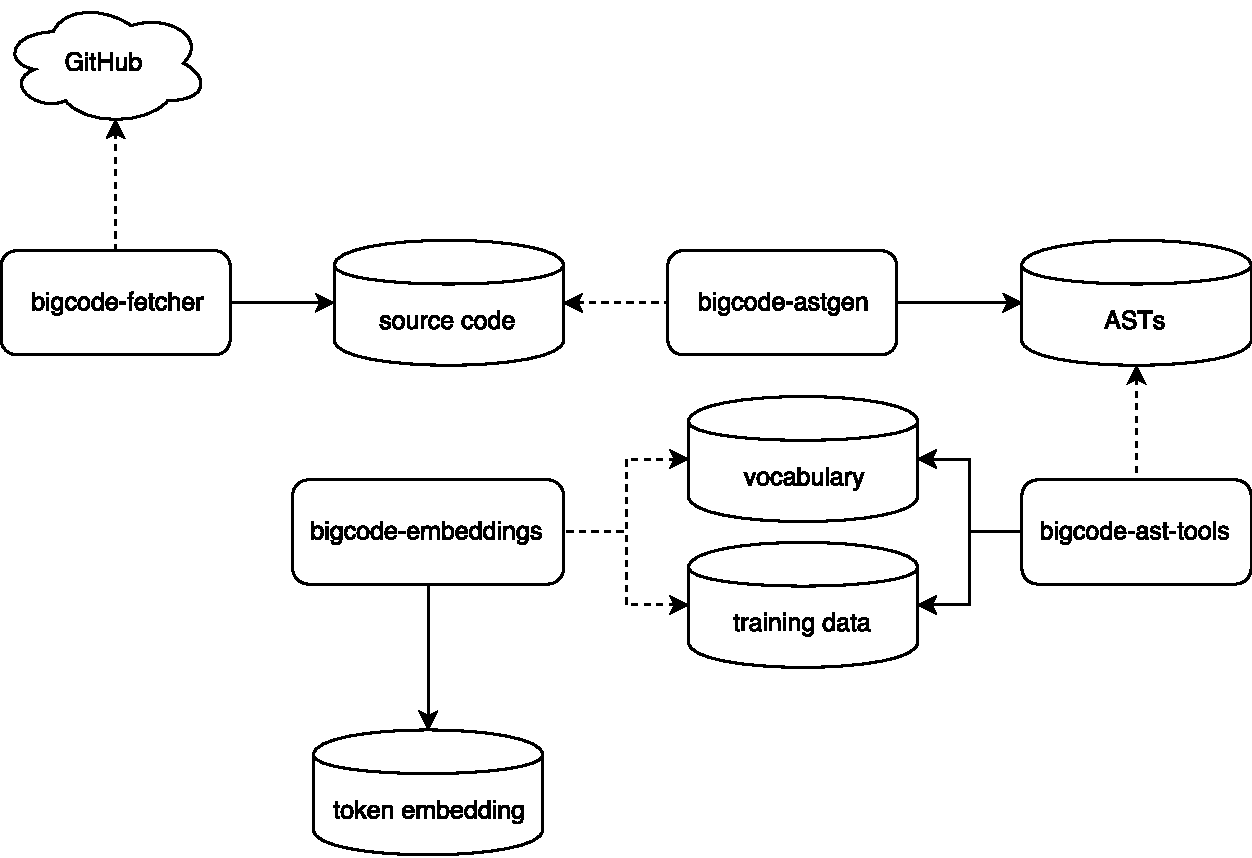
\includegraphics[width=14cm]{images/embedding-generation.pdf}
  \caption{\label{fig:embedding-generation} Embedding generation}
\end{figure}
%
\subsection{Vocabulary generation}
To be able to learn embedding for different tokens in a target programming
language, we first generate a finite set of tokens --- the vocabulary of the
programming language. There are a few different choices to consider when
generating the vocabulary of the language, the main choices we consider are:

\begin{enumerate}
\item Should application specific tokens be included in the vocabulary?
\item How large should be the vocabulary?
\end{enumerate}

We define application specific tokens as tokens that can be unique to a program,
for example, identifiers such as variable and method names or values in
literals.
If we choose to ignore the application specific tokens, we do not remove the
token but rather ignore its value and keep only its type.
We will consider the code snippet in listing~\ref{lis:is-minor} to explain how
we can treat application specific tokens.

\begin{figure}
  \lstinputlisting[
    language=Python,
    label=lis:is-minor,caption=\lstinline{is_minor} function in Python]
    {./snippets/is_minor.py}
\end{figure}

First, given we take all application specific tokens, we will have the following
tokens.

\begin{lstlisting}[numbers=none,language=Python]
def, is_minor, age, if, age, >=, 18, print, "you are major",
else, "you are minor"
\end{lstlisting}

On the other hand, if we decide to strip all the application specific tokens, we
will replace all the token with a value by their type, and therefore all
identifiers will be replaced by a common \lstinline{<ident>} token, all string
literals will be replaced by a common \lstinline{<string>} token, and only the
following tokens set will remain in the vocabulary.

\begin{lstlisting}[numbers=none,language=Python]
def, <ident>, if, <binary_op>, <string>, else
\end{lstlisting}

If we choose to ignore all application specific tokens, we only keep a
predictable number of tokens that the target programming language defined in its
specifications, and we can therefore ignore the size of the vocabulary issue
altogether as the number of tokens we might expect will always be small enough.

When using application specific tokens, although we could simply use all the
tokens as shown in the example above, all tokens might not be very significant
and we therefore need to choose what tokens we want to keep and what tokens we
want to ignore. As many identifiers can be found across applications, especially
the one found in the standard library or well-known libraries of a programming
language, we decide to keep all identifiers. However, we decide not to keep
string literals as these are too rarely shared between different programs.
Another issue when using application specific tokens is the case where a token
encountered after having generated our vocabulary does not exist in the
vocabulary, in which case it is not possible to map it directly to an index in
the vocabulary. A common approach to this issue in natural language processing
is to assign a special index which is used for all unknown tokens. However, in
our case, each token has a type and a value, we therefore decide to use the type
without its value if the type and value pair of the token cannot be found in the
vocabulary. This means that for every type in the target programming language,
we will have a token representing the type with no value in the vocabulary. When
looking up the token in the vocabulary, we first look for a token with the same
value and type. If we find one, we use its index, otherwise we fallback to
looking for the token with the same type instead and use its index. As there are
only a limited number of token types in a programming language, we are therefore
sure to at least find the matching type.

When using application specific tokens, the number of tokens will increase with
the number of files used to generate the vocabulary, and we therefore need to
set a threshold to the number of tokens we want to use. This threshold is set
experimentally, and given $n$ as this threshold, our vocabulary will be composed
of the $n$ most common tokens from the files that we used to generate the
vocabulary.

In algorithm~\ref{alg:generate-vocabulary}, we give a high-level overview of our
vocabulary generation algorithm and in algorithm~\ref{alg:lookup-token} we show
how we lookup a token in the vocabulary.

\begin{algorithm}
  \caption{\label{alg:generate-vocabulary}Vocabulary generation algorithm}
  \begin{algorithmic}[1]
    \Function{GenerateVocabulary}{\lstinline{sourceFiles},
      \lstinline{includeValues}, \lstinline{maxSize}}
      \State \lstinline{tokensCount} $\gets$ empty map
      \For{\lstinline{file} in \lstinline{sourceFiles}}
        \State \lstinline{tokens} $\gets$ \lstinline{tokenize(file)}
        \For{\lstinline{token} in \lstinline{tokens}}
          \If{\lstinline{(token.type, token.value)} $\notin$ \lstinline{tokensCount}}
            \State \lstinline{tokensCount[(token.type, token.value)]} $\gets$ 0
          \EndIf
          \State Increment \lstinline{tokensCount[(token.type, token.value)]}
          \If{\lstinline{includeValues}}
            \If{\lstinline{(token.type, null)} $\notin$ \lstinline{tokensCount}}
              \State \lstinline{tokensCount[(token.type, null)]} $\gets$ 0
            \EndIf
            \State Increment \lstinline{tokensCount[(token.type, null)]}
          \EndIf
        \EndFor
      \EndFor
      \State Sort \lstinline{tokensCount} by value
      \State \lstinline{vocabulary} $\gets$ first \lstinline{maxSize} keys of \lstinline{tokensCount}
      \State \lstinline{return vocabulary}
    \EndFunction%
  \end{algorithmic}
\end{algorithm}

\begin{algorithm}
  \caption{\label{alg:lookup-token}Token lookup}
  \begin{algorithmic}[1]
    \Function{LookupTokenIndex}{\lstinline{vocabulary}, \lstinline{token}}
      \If{(token.type, token.value) $\in$ vocabulary}
        \State \lstinline{return vocabulary.indexOf((token.type, token.value))}
      \EndIf
      \State \lstinline{return vocabulary.indexOf((token.type, null))}
    \EndFunction%
  \end{algorithmic}
\end{algorithm}

In algorithm~\ref{alg:generate-vocabulary}, \lstinline{sourceFiles} is a list of
source code files to use to generate the vocabulary, \lstinline{includeValues}
is a boolean that is \lstinline{true} if we want to use token values and
\lstinline{false} if we do not --- i.e. if we do not use anything application
specific. \lstinline{maxSize} is the maximum number of tokens in the generated
vocabulary. In algorithm~\ref{alg:lookup-token}, \lstinline{vocabulary} is the
vocabulary generated by \lstinline{GenerateVocabulary} and \lstinline{token} is
the token that needs to be lookup. It is worth noting that for algorithms
relying on this method to work in a reasonable time, \lstinline{indexOf} must
run in constant time $\mathcal{O}(1)$, and is therefore implemented using a
hash.
\subsection{Generating data to train skipgram model}
After generating the vocabulary, we need to generate data to train a skipgram
model, presented in~\ref{ssec:skipgram-model}. In the context of natural
language processing, the input is usually considered as a sequence, and the
context of a particular word is the words before and after this word in the
sequence of words used for training. Furthermore, the distance between the word
and its context is normally context by a single window size hyper-parameter.
We could apply the same approach by treating a program as a sequence of tokens,
but we decide to take advantage of the topological information contained by the
AST, we decide to work on the AST rather than on a simple sequence of token. We
therefore need to define the context of a word, or rather a token in our case,
differently than for a sequence.

In the context of a tree, a node is directly connected to its parent and its
children. We can therefore define parents and children to be the context of a
node. Depending on the use case, the siblings of a node could also be viewed as
a viable candidate its context. A single window size parameter could be used to
control how deep upward and downward should the context of a node be. However,
while a node will only have a single parent, it can have any number of children,
and therefore, while having a window size of $3$ for the ancestors would only
generate $3$ nodes in the context, if every descendant of a node had $5$
children, a window size of $3$ would generate $5^3 = 125$ nodes in the context,
which would probably generate more noise than signal when trying to train a
skipgram model. We therefore decide to use two different parameters to control
the window size of the ancestors and the window size of the descendant when
generating the data to train our skipgram model. When we do include siblings in
the context, we decide to only use the direct siblings of the nodes and not to
use the siblings of the ancestors, although this could also be another parameter
of the algorithm. In
algorithms~\ref{alg:generate-skipgram},~\ref{alg:generate-context}
and~\ref{alg:find-descendants}, we describe the algorithms we use to generate
the data to train a skipgram model.

\begin{algorithm}
  \caption{\label{alg:generate-skipgram}Data generation for skipgram model}
  \begin{algorithmic}[1]
    \Function{GenerateSkipgramData}{\lstinline{files}, \lstinline{vocabulary}, \lstinline{params}}
      \State \lstinline{skipgramData} $\gets \{\}$
      \For{\lstinline{file} in \lstinline{files}}
        \State \lstinline{ast} $\gets$ \lstinline{GenerateAST(file)}
        \For{\lstinline{node} in \lstinline{ast}}
          \State \lstinline{nodeIndex} $\gets$ \lstinline{LookupTokenIndex(node)}
          \State \lstinline{contextNodes} $\gets$
          \lstinline{GenerateContext(node, params)}
          \For{\lstinline{contextNode} in \lstinline{contextNodes}}
            \State \lstinline{contextNodeIndex} $\gets$
            \lstinline{LookupTokenIndex(contextNode)}
            \State \lstinline{skipgramData} $\overset{+}{\leftarrow}$ \lstinline{(nodeIndex, contextNodeIndex)}
          \EndFor%
        \EndFor%
      \EndFor%
      \State \lstinline{return skipgramData}
    \EndFunction%
  \end{algorithmic}
\end{algorithm}
%
\begin{algorithm}
  \caption{\label{alg:generate-context}Context generation for an AST node}
  \begin{algorithmic}[1]
    \Function{GenerateContext}{\lstinline{node}, \lstinline{params}}
      \State \lstinline{contextNodes} $\gets$ \lstinline{FindDescendants(node, params.descendantWindowSize, 0)}
      \State \lstinline{parent} $\gets$ \lstinline{node.parent}
      \State \lstinline{n} $\gets$ 0
      \While{\lstinline{parent} is defined $\land$ \lstinline{n} $<$ \lstinline{params.ancestorWindowSize}}
        \State \lstinline{contextNodes} $\overset{+}{\leftarrow}$ \lstinline{parent}
        \State \lstinline{parent} $\gets$ \lstinline{parent.parent}
        \State \lstinline{n} $\gets$ \lstinline{n + 1}
      \EndWhile
      \If{\lstinline{params.includeSiblings} $\land$ \lstinline{node.parent}
        is defined}
        \For{\lstinline{sibling} in \lstinline{node.parent.children}}
          \State \lstinline{contextNodes} $\overset{+}{\leftarrow}$ \lstinline{sibling}
        \EndFor
      \EndIf
      \State \lstinline{return contextNodes}
    \EndFunction%
  \end{algorithmic}
\end{algorithm}
%
\begin{algorithm}
  \caption{\label{alg:find-descendants}Find descendants for a node until given depth}
  \begin{algorithmic}[1]
    \Function{FindDescendants}{\lstinline{node}, \lstinline{maxDepth}, \lstinline{currentDepth}}
      \If{\lstinline{currentDepth} $\geq$ \lstinline{maxDepth}}
        \State \lstinline{return} $\{\}$
      \EndIf
      \State \lstinline{descendants} $\gets$ \lstinline{node.children}
      \For{\lstinline{child} in \lstinline{node.children}}
        \State \lstinline{childDescendants} $\gets$ \lstinline{FindDescendants(child, maxDepth, currentDepth+1)}
        \State \lstinline{descendants} $\gets$ \lstinline{descendants} $\cup$ \lstinline{childDescendants}
      \EndFor
      \State \lstinline{return children}
    \EndFunction
  \end{algorithmic}
\end{algorithm}
%
Algorithm~\ref{alg:generate-skipgram} takes as input a list of files written in
the programming language for which we want to generate token embedding, the
vocabulary extracted for this programming language and the parameters described
above. It loops over all the nodes in the file, and uses
algorithms~\ref{alg:generate-context} and~\ref{alg:find-descendants} to find all
nodes in the context of the current node, and returns a list of pair of indexes
where each pair represent a target node and a node in its context.
Algorithm~\ref{alg:generate-context} takes as input a node and the parameters
described above, and returns the set of nodes in the context of the given node.
It first uses algorithm~\ref{alg:find-descendants} to find all the descendants
of the node in the window given by the passed parameters, then find all the
ancestors in the given window and finally add the siblings to the set of results
if necessary. Algorithm~\ref{alg:find-descendants} takes a node, the maximum
depth up to which descendants should be populated and the current depth ---
which will initially be set to 0 --- and returns the set of descendants up to
the passed maximum depth for the node. It first adds all the children of the
current node to the set of descendants, then recurses through all the children
until the current depth is equal to the maximum depth for which to generate
descendants.
\subsection{Training a skipgram model}
Once the data is generated using
algorithms~\ref{alg:generate-skipgram},~\ref{alg:generate-context}
and~\ref{alg:find-descendants}, the last step needed to generate embedding is to
actually train a skipgram model using the generated data.
Algorithm~\ref{alg:generate-skipgram} generates pairs of indexes which can be
directly fed to a neural network, and there is therefore no need for further
pre-processing. To train the model, the vocabulary used is the same as the one
used to generate the skipgram data and the size of the embedding is a hyper
parameter of the model. The model is trained using a negative sampling objective
shown in equation~\ref{eq:negative-sampling} as given
in~\cite{DBLP:journals/corr/MikolovSCCD13}.
%
\begin{equation}
  \label{eq:negative-sampling}
  \log \sigma \left({v'_{w_O}}^T v_{w_I} \right) + \sum_{i=1}^k \mathbb{E}_{w_i \sim P_n(w)}
  \left[ \log \sigma\left( {v'_{w_i}}^T v_{w_I} \right) \right]
\end{equation}
%
In equation~\ref{eq:negative-sampling}, $v$ are the weights of the hidden
layer, which will be used as embedding, $v'$ are the weights of the output
layer, $w_I$ is an input token and $w_O$ is a token in its context. $w_i$ are
the ``noise'' tokens which are randomly sampled from the vocabulary using a
noise distribution $P_n$, for which we use a unigram distribution for reasons
described in~\cite{DBLP:journals/corr/MikolovSCCD13}.
